\begin{spacing}{1.3}
   
    \section{DP over Interval}

    In this topic, we are going to talk about a specific type of DP: 
    {\bf DP over intervals}. As indicated by its name, the DP problems we will see 
    is to find the optimal solution over an interval(for example, over interval $[i,j]$)
    and the algorithms will fill in the DP table from smallest interval size, such as 
    interval length equals to 1, to largest interval size, such as interval $[1,n]$.


    \vspace{0.3in}
    \section{Longest Palindromic Substring}

    \begin{definition}
        A {\bf palindrome} is a string that reads the same backward and forward.
        For example, ``radar'', ``level'', ``madam''.
    \end{definition}

    Our problem is that given a string $X=x_1x_2\cdots x_n$, where $x_i$ represents $i$-th 
    character, we want to find the {\bf longest palindromic substring}. 
    Here {\bf substring} means they must be {\it consecutive}.

    For example, given string $X={\tt ACCABA}$, there are {\tt CC, ACCA, ABA} 
    three {\bf palindromic substrings}, and the longest one is {\tt ACCA}.

    This is a typical problem of dp over interval, since among all substrings, which 
    can be regarded as the characters in interval $X[i\cdots j]$, we want to decide 
    if it is a palindrome. A brute force algorithm should takes $O(n^3)$ time, 
    by using $O(n^2)$ time to loop over $i$ and $j$, and use another $O(n)$ time for 
    checking.

    However, the brute force algorithm can, obviously, be improved, since 
    it calculates a lot of redundant things. For example, if we know $X[3\cdots 6]$
    is a palindrome, and to check whether $X[2\cdots 7]$ is, we only need 
    to check whether $X[2]$ equals to $X[7]$, no need to again, loop over all elements
    between. This is where our DP algorithm improves from the brute force algorithm.

    We define $p[i,j]$ be {\tt true} if $X[i\cdots j]$ is a palindrome.(See? 
    That's ``over interval'', since we care about the solution over an interval $[i,j]$)

    Inspired by the example above, to check if $p[i,j]$ is a palindrome, we can check 
    if both $X[i]=X[j]$ and $p[i+1, j-1]=true$ holds, i.e., the leftmost character is 
    the same as the rightmost character, and the substring except for them two 
    is a palindrome. To write it as a recurrence,
    $$p[i,j]=true\ \ \   {\rm if\ } x_i=x_j {\ \rm and\ } p[i+1, j-1]=true$$

    Now we need to consider extreme cases, or initial conditions. Above, we first 
    check if the leftmost character is the same as the rightmost character, and then 
    the substring in the middle, but what if the string has only 1 or 2 characters?
    That's the initial condition:
    \begin{align*}
        p[i,i] = true &\ \   {\rm for \ all}\ i\\ 
        p[i, i+1] = true &\ \   {\rm if \ } x_i=x_{i+1}
    \end{align*}

    Now we can fill in the DP table according to our recurrence.
    \begin{figure}[htbp]
        \centering
        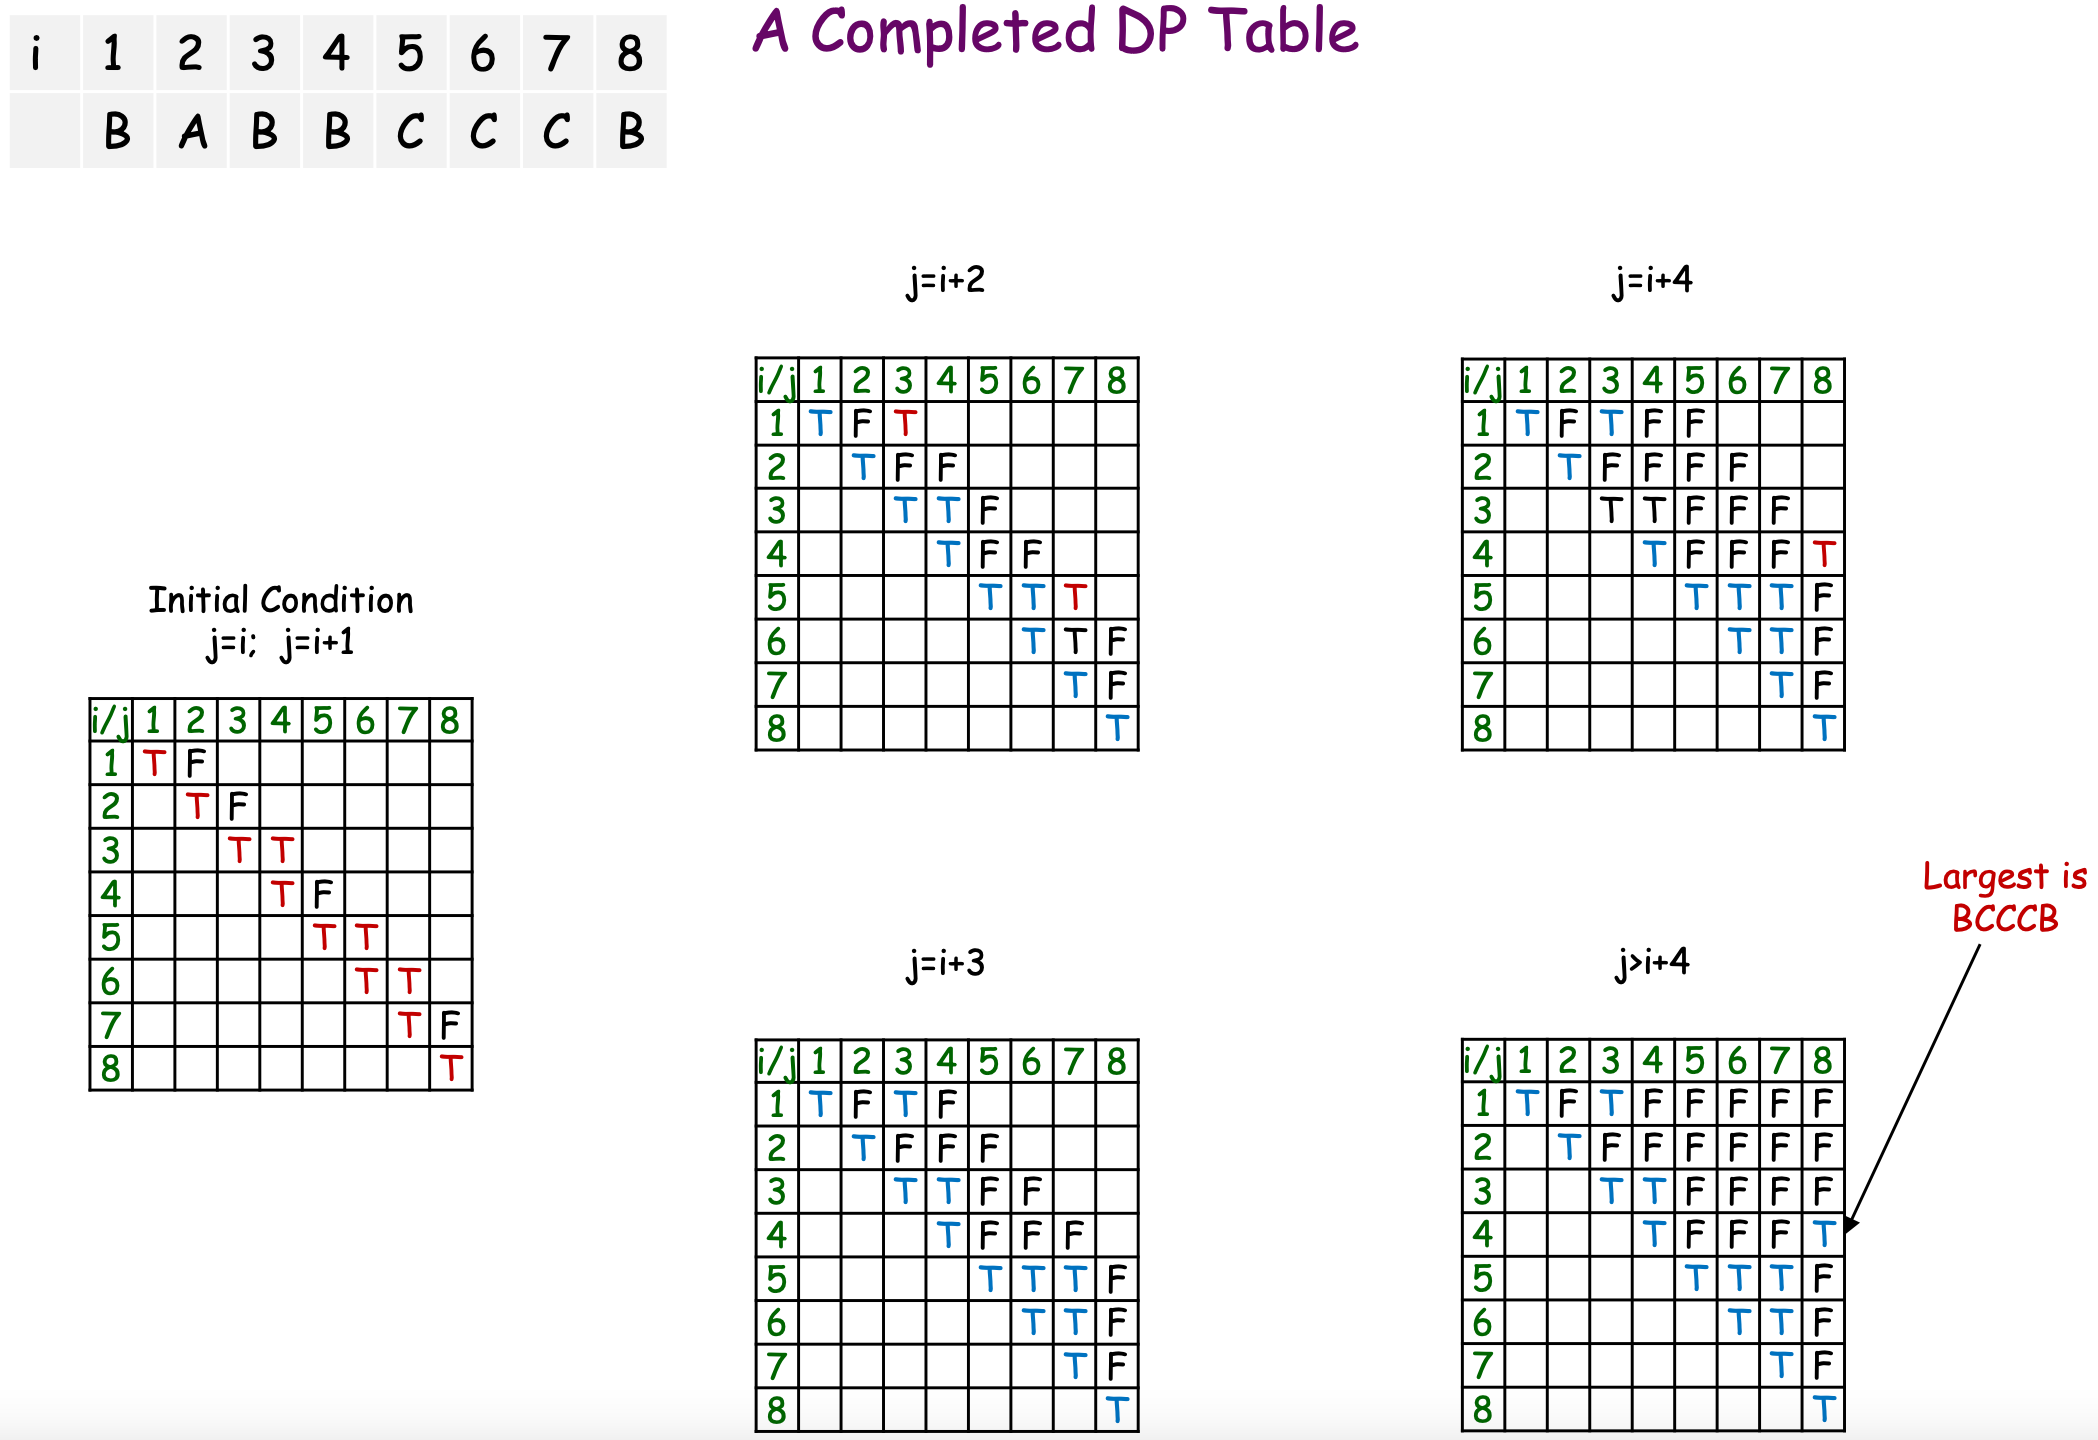
\includegraphics[scale=0.37]{images/10-palin-table.png}
    \end{figure}

    As shown in tables above, we fill in the tables, and at the same time, 
    records the max palindrome's length we've ever met.
    The pseudocode is given below.
    \begin{algorithm*}[htbp]
        \caption{Longest-Palindrome($X$)}
        $maxLen\lar 1$\qquad \tcp{one letter is also palindrome}

        \For{$i\lar 1$ to $n-1$}{
            $p[i,i]\lar true$ \qquad \tcp{initial condition 1}

            \eIf{$X_i=X_{i+1}$}{
                $p[i, i+1]\lar true$ \qquad \tcp{initial condition 2}

                $maxLen\lar 2$ \qquad \tcp{met parlindrome of length 2}
            }{
                $p[i, i+1]\lar false$
            }
        }

        \tcp{$l$ loops over interval length, $l$ stands for ``length''}
        \For{$l\lar 3$ to $n$}{
            \tcp{$i$ loops over left endpoint of interval}
            \For{$i\lar 1$ to $n-l+1$}{
                $j\lar i+l-1$\qquad \tcp{$j$ is the right endpoint of interval}

                \eIf{$p[i+1, j-1]=true$ and $X_i=X_j$}{
                    $p[i,j]\lar true$

                    \tcp{since we loop over interval length from small to large, 
                    here $l$ is AT LEAST $maxLen$, so no need to check}
                    $maxLen \lar l$ 
                }{
                    $p[i,j]\lar false$
                }
            }
        }
        return $maxLen$
    \end{algorithm*}

    The running time of this algorithm is $O(n^2)$ since there are two nested loops, each 
    has order $n$. 
    
    The space complexity is $O(n^2)$, but notice that each time when we 
    check whether a length $l$ substring is a palindrome, we only refer to 
    the previous records of length $l-2$, so it is possible that we can only 
    store records of length $l-2$ and $l-1$ when we check length $l$ intervals,
    which can improve the space complexity to $O(n)$. (It will become 
    clearer if you fill in the DP table by hand)

\end{spacing}